% =============================================================================
% Phase I report - SIMD Vector Processing Unit
% Build:  make report
%   (runs reports/src/make_figures.py for the result plots, then tectonic)
% The diagrams are TikZ files in figures/, drawn in the same font as the text.
% =============================================================================
\documentclass[journal]{IEEEtran}
\usepackage[T1]{fontenc}
\usepackage{graphicx}
\usepackage{booktabs}
\usepackage{array}
\usepackage{amsmath}
\usepackage{cite}
\usepackage{url}
\usepackage{xcolor}
\usepackage{listings}
\usepackage{tikz}
\usetikzlibrary{arrows.meta, positioning, fit, backgrounds, decorations.pathreplacing}
\usepackage[hidelinks]{hyperref}

% ---- Colours shared by every diagram and plot --------------------------------
% blue = vector / SIMD side, orange = scalar side, grey = control and memories
\definecolor{simd}{HTML}{3F7FDC}     \definecolor{simdfill}{HTML}{E9F1FC}
\definecolor{scal}{HTML}{EF6F3C}     \definecolor{scalfill}{HTML}{FDEEE7}
\definecolor{edge}{HTML}{6F6E69}     \definecolor{greyfill}{HTML}{F4F4F3}
\tikzset{
  box/.style={draw=edge, rounded corners=2pt, fill=white, align=center, inner sep=2pt, line width=0.5pt},
  arr/.style={-{Stealth[length=1.6mm, width=1.2mm]}, draw=edge, line width=0.6pt},
  note/.style={font=\scriptsize, text=edge},
}

\lstset{basicstyle=\ttfamily\footnotesize, columns=flexible, keepspaces=true, frame=single,
        framerule=0.3pt, rulecolor=\color{edge}, xleftmargin=2pt, xrightmargin=2pt,
        commentstyle=\color{edge}, morecomment=[l]{\#}}

\newcommand{\x}{\ensuremath{\times}}
\newcolumntype{L}[1]{>{\raggedright\arraybackslash}p{#1}}

\begin{document}

\title{Design and Evaluation of a Parameterised\\SIMD Vector Processing Unit on FPGA}

\author{Mahir Abdullah, Krishiv Gupta, Abhiman Singh, Gogulamudi Jayadeep, and Ashish Kushwaha%
\thanks{This work forms Phase I of Project 11, SIMD Vector Processing Unit, November 2026.
The authors are with Newton School of Technology, Rishihood University.}%
\thanks{Code, data and all reported results are available at
\url{https://github.com/mahir-m01/SIMD-Vector-Processing-Unit}.}}

\markboth{Design and Evaluation of a Parameterised SIMD Vector Processing Unit on FPGA}%
{Design and Evaluation of a Parameterised SIMD Vector Processing Unit on FPGA}

\maketitle

% =============================================================================
\begin{abstract}
Signal processing, graphics and machine learning apply the same arithmetic to long
arrays of numbers. Single-instruction, multiple-data (SIMD) hardware exploits this
regularity: one instruction drives several arithmetic lanes at once. We present the
Phase~I design of a small SIMD vector processing unit in Verilog whose lane count is
a parameter. At eight lanes it holds eight 128-bit vector registers of eight 16-bit
elements, replicates a 14-operation lane ALU, broadcasts a scalar operand through
per-lane multiplexers and sums the lanes in an adder tree, so that a dot-product step
is one instruction. With one lane the same RTL becomes a scalar processor that runs
the same programs with the same 48-instruction ISA and timing rules, which gives a
like-for-like baseline. An instruction-level golden model predicts every result and
the exact cycle count; unit, system, directed, random-program and board testbenches
compare the hardware with it, and deliberately injected bugs confirm that the tests
catch faults. Every run, including 4,000 random programs, matches the model exactly
for 1, 2, 4 and 8 lanes. On five kernels of 256
elements, eight lanes need $7.87$--$7.92\x$ fewer clock cycles than one, 1.0--1.7\%
below ideal, and the shortfall is the serial set-up code predicted by Amdahl's law.
Built with every instruction in use and placed and routed on a Lattice ECP5-25F, the
eight-lane unit uses 22.2\% of the logic cells, and its estimated maximum clock is
29.1~MHz against 43.3~MHz for one lane, so the wall-clock speed-up is $5.3\x$ and
throughput rises from 5.6 to 29.9 million elements per second.
\end{abstract}

\begin{IEEEkeywords}
Data-level parallelism, FPGA, golden model, hardware verification, SIMD, vector
processor, Verilog.
\end{IEEEkeywords}

% =============================================================================
\section{Introduction}

\IEEEPARstart{A}{} scalar processor spends most of its effort on control: fetching,
decoding and sequencing each instruction. When a program adds two arrays, that effort
is repeated for every element, although every element needs the same work. A SIMD
processor issues one instruction for a group of elements. The control cost is paid
once and the arithmetic is replicated across \emph{lanes}. This is
\emph{data-level parallelism}, the form of parallelism behind vector
supercomputers~\cite{cray1}, multimedia instruction-set extensions~\cite{mmx} and
graphics processors~\cite{hp6}.

\textbf{Problem statement.} The project asks for a small SIMD unit that performs
identical arithmetic and logic operations in parallel, built from a vector register
file, parallel ALUs, a vector control unit, lane multiplexers, a result combiner and
an optional scalar interface. Scalar and SIMD versions of the same workload must be
compared, the vector results verified, and cycle counts, throughput, FPGA resources
and maximum frequency measured. We answer three questions with measurements:
\begin{enumerate}
\item How close to the ideal $L\x$ does an $L$-lane unit come in clock cycles?
\item What does each extra lane cost in FPGA logic, multipliers and memory?
\item How much does the wider datapath slow the clock, and what wall-clock speed-up
      remains?
\end{enumerate}

This paper reports Phase~I of a two-phase project. Its contributions are:
\begin{itemize}
\item a synthesizable SIMD unit in Verilog whose lane count is a parameter, with every
      block named in the brief (Section~\ref{sec:design});
\item a 48-instruction ISA, an assembler and an instruction-level golden model that
      predicts results and exact cycle counts (Sections~\ref{sec:isa}
      and~\ref{sec:tools});
\item a layered verification flow with self-checking testbenches, directed corner
      tests, random programs, a board-level check and mutation tests
      (Section~\ref{sec:verif});
\item a scalar-versus-SIMD comparison on five kernels and an FPGA resource and
      frequency sweep over 1, 2, 4 and 8 lanes (Section~\ref{sec:results}).
\end{itemize}

Section~\ref{sec:lit} reviews related work. Section~\ref{sec:design} describes the
design, its tools and its verification, and Section~\ref{sec:results} presents the
results. Section~\ref{sec:discussion} discusses them and their limits, and
Section~\ref{sec:conclusion} concludes with the Phase~II plan. Fig.~\ref{fig:flow}
gives an overview of the flow that produces every result.

\begin{figure*}[t]
\centering
% Fig. 1 - the Phase I flow: how every result in the report is produced.
% Top row: correctness and cycle counts. Bottom row: hardware cost and clock.
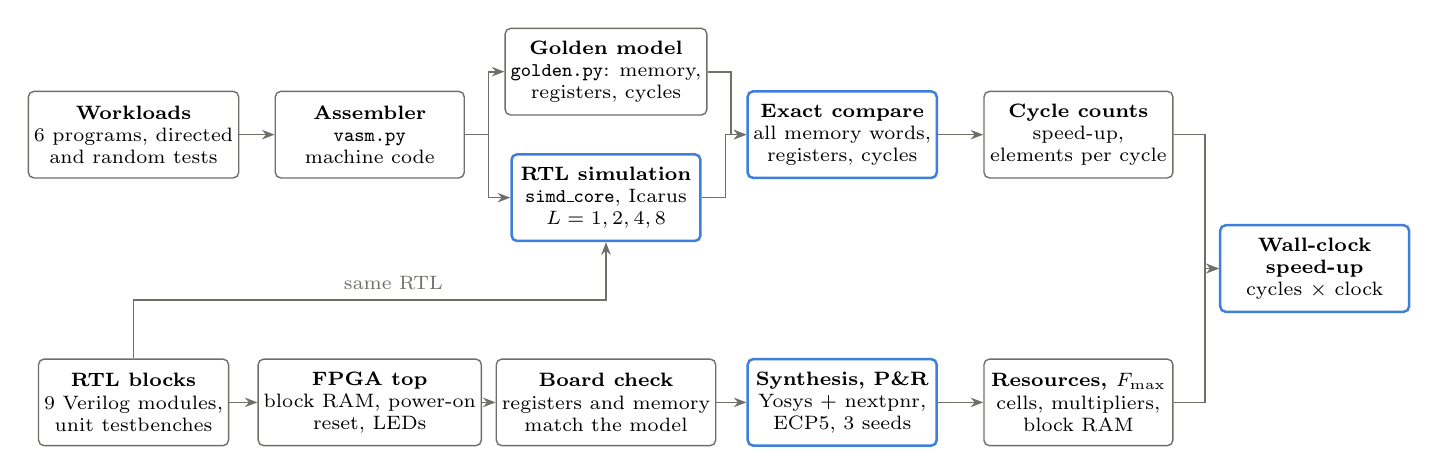
\begin{tikzpicture}[x=1mm, y=1mm, font=\scriptsize,
    stage/.style={box, minimum width=24mm, minimum height=11mm},
    key/.style={stage, draw=simd, line width=0.9pt}]

% ---- Top row: simulation ------------------------------------------------------
\node[stage] (prog) at (0,0)    {\textbf{Workloads}\\6 programs, directed\\and random tests};
\node[stage] (asm)  at (30,0)   {\textbf{Assembler}\\\texttt{vasm.py}\\machine code};
\node[stage] (gold) at (60,8)   {\textbf{Golden model}\\\texttt{golden.py}: memory,\\registers, cycles};
\node[key]   (rtl)  at (60,-8)  {\textbf{RTL simulation}\\\texttt{simd\_core}, Icarus\\$L = 1, 2, 4, 8$};
\node[key]   (cmp)  at (90,0)   {\textbf{Exact compare}\\all memory words,\\registers, cycles};
\node[stage] (cyc)  at (120,0)  {\textbf{Cycle counts}\\speed-up,\\elements per cycle};

% ---- Bottom row: hardware ----------------------------------------------------------
\node[stage] (mods) at (0,-34)  {\textbf{RTL blocks}\\9 Verilog modules,\\unit testbenches};
\node[stage] (top)  at (30,-34) {\textbf{FPGA top}\\block RAM, power-on\\reset, LEDs};
\node[stage] (brd)  at (60,-34) {\textbf{Board check}\\registers and memory\\match the model};
\node[key]   (pnr)  at (90,-34) {\textbf{Synthesis, P\&R}\\Yosys + nextpnr,\\ECP5, 3 seeds};
\node[stage] (res)  at (120,-34){\textbf{Resources, $F_{\max}$}\\cells, multipliers,\\block RAM};

% ---- Where the two rows meet -------------------------------------------------------
\node[key] (wall) at (150,-17)  {\textbf{Wall-clock}\\\textbf{speed-up}\\cycles $\times$ clock};

\draw[arr] (prog) -- (asm);
\draw[arr] (asm.east) -- ++(3,0) |- (gold.west);
\draw[arr] (asm.east) -- ++(3,0) |- (rtl.west);
\draw[arr] (gold.east) -- ++(3,0) |- (cmp.west);
\draw[arr] (rtl.east) -- ++(3,0) |- (cmp.west);
\draw[arr] (cmp) -- (cyc);
\draw[arr] (cyc.east) -- ++(4,0) |- (wall.west);
\draw[arr] (res.east) -- ++(4,0) |- (wall.west);

\draw[arr] (mods) -- (top);
\draw[arr] (top) -- (brd);
\draw[arr] (brd) -- (pnr);
\draw[arr] (pnr) -- (res);
\draw[arr] (mods.north) -- (0,-21) -- node[note, above, pos=0.55] {same RTL} (60,-21) -- (rtl.south);
\end{tikzpicture}

\caption{Phase I flow. Top: each program is assembled once and run on the golden model
and on the RTL core at every lane count; memory, registers, instruction count and cycle
count must match exactly. Bottom: the same RTL is wrapped with block-RAM memories,
checked from power-on in simulation, then placed and routed for resources and maximum
clock frequency. Cycle counts and clock frequency together give the wall-clock speed-up.}
\label{fig:flow}
\end{figure*}

% =============================================================================
\section{Literature Review}\label{sec:lit}

\textbf{Taxonomy and vector machines.} Flynn's taxonomy~\cite{flynn72} classifies
machines by the number of instruction and data streams; SIMD names one instruction
stream acting on many data elements. The first commercially successful SIMD designs
were vector supercomputers such as the Cray-1~\cite{cray1}, whose vector registers and
pipelined functional units let one instruction process up to 64 elements, hiding memory
latency and avoiding the issue cost of a scalar loop. Espasa~\emph{et
al.}~\cite{espasa98} review the history of vector architectures and argue that their
strengths, few instructions per unit of work and simple control, suit multimedia
workloads. Hennessy and Patterson~\cite{hp6} trace the same principles from
vector machines to subword SIMD and GPUs.

\textbf{Subword SIMD in general-purpose processors.} Intel MMX~\cite{mmx} introduced
\emph{packed} data types: one 64-bit register treated as eight bytes or four 16-bit
words, with one instruction operating on all of them. Streaming SIMD Extensions
(SSE)~\cite{sse} widened the registers to 128 bits, the width also used by Arm Neon.
Two conventions from this line of work are adopted directly here: compare instructions
that write all-ones or all-zeros masks, so that conditionals need no branch, and a
fixed 128-bit register divided into lanes.

\textbf{Scalable vector architectures.} VIRAM~\cite{viram} showed that a vector
architecture with lanes scales across embedded media workloads more simply than
superscalar or VLIW designs, and that a compiler can vectorise most kernels
automatically. Asanovi\'c~\cite{asanovic98} analysed lane-based vector microprocessors
in depth, and Lee~\emph{et al.}~\cite{maven} found vector cores more efficient than
MIMD, subword-SIMD and SIMT designs even on fairly irregular kernels. Two current ISAs
leave the vector length to the implementation: the RISC-V vector extension~\cite{rvv}
and the Arm Scalable Vector Extension, which allows registers from 128 to 2048 bits
under one vector-length-agnostic programming model~\cite{sve}. Ara~\cite{ara}
implements RISC-V V with identical lanes, each holding a slice of the vector register
file, and reaches over 1~GHz in 22-nm technology. The lane replication used in this
project follows the same idea at a much smaller scale.

\textbf{Current SIMD instruction sets.} Table~\ref{tab:isas} compares this unit with
instruction sets in use today. Intel SSE2 and AVX2~\cite{intelsdm}, Arm
Neon~\cite{armarm} and the MIPS SIMD Architecture (MSA)~\cite{msa} fix the register
width in the ISA; RISC-V V lets one binary run on any width through \texttt{vsetvli}.
Three conventions are adopted here. The 128-bit register and the all-ones compare mask
follow SSE, Neon and MSA. The vector--scalar form follows RISC-V V's \texttt{.vx}
instructions, which broadcast a scalar register inside the instruction. A full sum
across lanes follows Neon's \texttt{ADDV} and RISC-V V's \texttt{vredsum}, whereas x86
\texttt{PMADDWD} and MSA \texttt{DOTP\_S} only add products in pairs; those two keep
each product at 32 bits, while \texttt{VDOT} keeps its low 16 bits.

\begin{table}[t]
\centering
\caption{SIMD Instruction Sets Compared}
\label{tab:isas}
\footnotesize
\setlength{\tabcolsep}{4pt}
\begin{tabular}{lllll}
\toprule
ISA & Width (bits) & Regs & Int.\ elements & Sum across lanes \\
\midrule
SSE2       & 128           & 8/16 & 8--64 & pairs (\texttt{PMADDWD}) \\
AVX2       & 256           & 16   & 8--64 & pairs (\texttt{VPMADDWD}) \\
Neon (A64) & 128           & 32   & 8--64 & full (\texttt{ADDV}) \\
MIPS MSA   & 128           & 32   & 8--64 & pairs (\texttt{DOTP\_S}) \\
RISC-V V   & \texttt{VLEN} & 32   & 8--64 & full (\texttt{vredsum}) \\
This work  & $16L$ (128)   & 8    & 16    & full, 16-bit products \\
\bottomrule
\end{tabular}
\end{table}

\textbf{Soft vector processors on FPGAs.} FPGAs suit lane-replicated designs because
the lane count can be matched to the device. VESPA~\cite{vespa} showed a soft vector
processor whose lane count and width can be scaled and customised to each application.
VIPERS~\cite{vipers} used a soft vector unit as a general-purpose accelerator for a
Nios~II processor and reported up to $44\x$ speed-up over a Nios~II/s with 32 lanes, at
$26\x$ its area. VEGAS~\cite{vegas} replaced the
vector register file with a scratchpad and introduced fracturable ALUs, and the
VectorBlox MXP~\cite{mxp} turned these ideas into a commercial core with 1 to over 128
ALUs. Vicuna~\cite{vicuna} is an open-source RISC-V vector coprocessor designed so that
its execution time is predictable, which allows tight worst-case timing analysis.
Most of these works report speed-up against a separate host processor, so the baseline
differs from the vector unit in microarchitecture as well as in width.

\textbf{Performance limits.} Amdahl's law~\cite{amdahl} bounds the speed-up of any
parallel unit by the fraction of work that stays serial; in a vector loop that
fraction is the set-up code, the loop control and the final reduction. Gustafson's
observation~\cite{gustafson} that larger problems shrink the serial fraction explains
why speed-up grows with array length. 

\textbf{Verification and tools.} Comparing a design against an independent
instruction-level model is standard practice in processor verification, and mutation
testing~\cite{demillo} judges a test suite by whether it detects deliberately injected
faults. Open-source flows make resource and timing results reproducible: Icarus
Verilog~\cite{icarus} simulates, Verilator~\cite{verilator} lints, and
Yosys~\cite{yosys} with nextpnr~\cite{nextpnr} synthesise, place and route designs for
the Lattice ECP5 using documented timing models.

\textbf{Gap addressed.} Published soft vector processors are large and are usually
compared against a different scalar core. This project builds a design small enough
for every line to be explained and verified. Its scalar baseline is the \emph{same}
RTL with one lane, so any measured gain comes from data-level parallelism alone, and
its timing is as predictable as Vicuna's in a far simpler form: the cycle count of
every program follows from its instruction and load counts.

% =============================================================================
\section{Proposed Solution}\label{sec:design}

\subsection{Design Goals and Parameters}
The design favours clarity over speed. Every instruction except a load completes in one
clock cycle, so there are no pipeline hazards and the cycle count of a program is exact.
Two parameters set the shape (Table~\ref{tab:params}): the number of lanes $L$ and the
element width $W = 16$ bits. With $L = 8$ a vector holds $8 \times 16 = 128$ bits, the
width of SSE and Neon (Fig.~\ref{fig:lanes}). The memories sit outside the core, so the
same RTL is used in simulation and on the FPGA. The RTL is plain Verilog (IEEE 1364-2005~\cite{ieee1364}):
one module per block, \texttt{generate} loops for the lanes and no vendor primitives.

\begin{table}[t]
\centering
\caption{Design Parameters}
\label{tab:params}
\footnotesize
\begin{tabular}{llL{0.48\columnwidth}}
\toprule
Parameter & Value & Meaning \\
\midrule
\texttt{LANES} ($L$) & 1, 2, 4, 8 & lanes in parallel (default 8) \\
\texttt{W}           & 16         & bits per element (signed) \\
vector registers     & $8 \times 16L$ bits & \texttt{v0}--\texttt{v7} \\
scalar registers     & $8 \times 32$ bits  & \texttt{s0}--\texttt{s7}, \texttt{s0} always 0 \\
\texttt{IADDR\_W}    & 8          & 256 instructions \\
\texttt{DADDR\_W}    & 10         & 1,024 data words (also on the FPGA) \\
\bottomrule
\end{tabular}
\end{table}

\begin{figure}[t]
\centering
% Fig. 2 - one SIMD instruction: VADD adds eight pairs of 16-bit numbers at once.
% Each column is a lane; nothing crosses from one lane to the next.
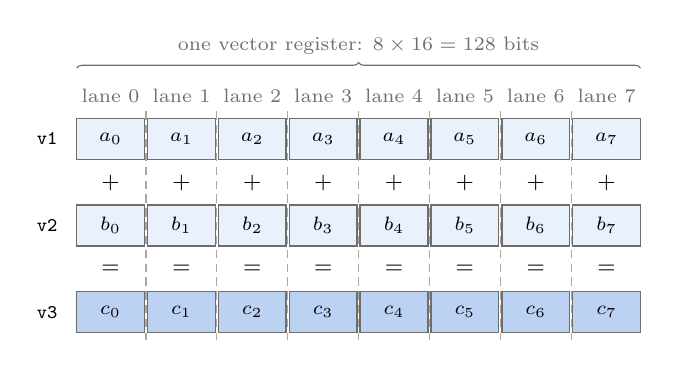
\begin{tikzpicture}[x=1mm, y=1mm, font=\scriptsize,
    cell/.style={draw=edge, minimum width=8.6mm, minimum height=5.2mm, inner sep=0pt, line width=0.5pt},
    vin/.style={cell, fill=simdfill},
    vout/.style={cell, fill=simd!35}]

% Lane labels and the three vector registers (lane 0 on the left).
\foreach \i in {0,...,7} {
  \node[note] at (\i*9, 19.5) {lane \i};
  \node[vin]  (a\i) at (\i*9, 14) {$a_{\i}$};
  \node[font=\footnotesize] at (\i*9, 8.4) {$+$};
  \node[vin]  (b\i) at (\i*9, 3) {$b_{\i}$};
  \node[font=\footnotesize] at (\i*9, -2.6) {$=$};
  \node[vout] (c\i) at (\i*9, -8) {$c_{\i}$};
}
\node[anchor=east] at (-5.5, 14) {\texttt{v1}};
\node[anchor=east] at (-5.5, 3)  {\texttt{v2}};
\node[anchor=east] at (-5.5, -8) {\texttt{v3}};

% Lane boundaries: no carry crosses them.
\foreach \i in {0,...,6}
  \draw[edge!60, densely dashed, line width=0.4pt] (\i*9+4.5, 17.5) -- (\i*9+4.5, -11.5);

% Width braces above v1.
\draw[decorate, decoration={brace, amplitude=2pt}, edge] (-4.3, 23) -- node[note, above=1.5pt] {one vector register: $8 \times 16 = 128$ bits} (67.3, 23);

\end{tikzpicture}

\caption{One SIMD instruction. A 128-bit register holds eight 16-bit elements, one per
lane, and \texttt{VADD} adds all eight pairs at once. Lanes are independent: no carry
crosses a lane boundary (dashed). The scalar build ($L = 1$) runs the same program with
one element per register.}
\label{fig:lanes}
\end{figure}

\subsection{Instruction Set}\label{sec:isa}
Instructions are 32 bits: a 6-bit opcode, three 3-bit register fields and a signed
16-bit immediate (Fig.~\ref{fig:format}). The two top opcode bits select one of four
classes (Table~\ref{tab:isa}); in the first three, the low four bits select one of 14
ALU jobs: \texttt{ADD}, \texttt{SUB}, \texttt{AND}, \texttt{OR}, \texttt{XOR}, three
shifts (\texttt{SLL}, \texttt{SRL}, \texttt{SRA}, by $b \bmod 16$), \texttt{MUL} (low
16 bits), \texttt{SEQ}, \texttt{SLT}, \texttt{SLTU}, \texttt{MIN} and \texttt{MAX}.
Fourteen jobs in three forms plus six memory, scalar and control instructions give 48
instructions. Compare jobs write \texttt{0xFFFF} for true and 0 for false, so a result
can be used directly as a mask with \texttt{VAND}. Arithmetic wraps around on overflow
($32767 + 1 = -32768$). Data addresses wrap modulo the memory size and the program counter wraps after
255. Unused opcodes in the three ALU classes write 0 to their destination, and the
others do nothing for one cycle, so every bit pattern has a defined effect.

\begin{figure}[t]
\centering
% Fig. 3 - the 32-bit instruction word, with four real encodings from vasm.py.
% One bit = 1.8 mm. Field values under each box are binary (imm in hex).
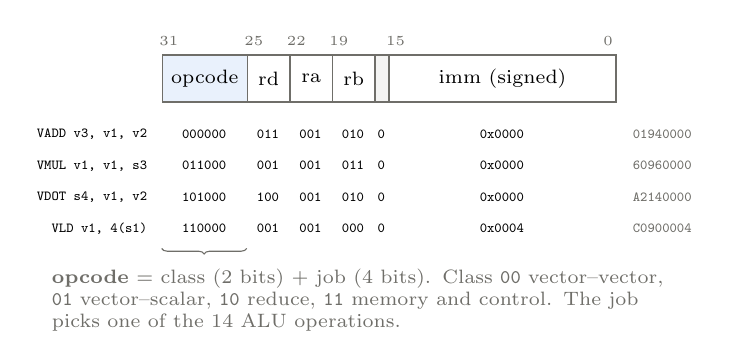
\begin{tikzpicture}[x=1mm, y=1mm, font=\scriptsize,
    field/.style={draw=edge, minimum height=6mm, inner sep=0pt, line width=0.5pt, anchor=south west},
    bits/.style={font=\tiny, text=edge},
    val/.style={font=\tiny\ttfamily}]

% Field boxes: (left edge, width, label, fill)
\foreach \x/\w/\t/\f in {0/10.8/opcode/simdfill, 10.8/5.4/rd/white, 16.2/5.4/ra/white,
                         21.6/5.4/rb/white, 27/1.8/{}/greyfill, 28.8/28.8/{imm (signed)}/white}
  \node[field, minimum width=\w mm, fill=\f] at (\x,0) {\t};

% Bit numbers: the top bit of each field, and bit 0.
\foreach \x/\b in {0.9/31, 11.7/25, 17.1/22, 22.5/19, 29.7/15, 56.7/0}
  \node[bits] at (\x, 7.8) {\b};

% Four encodings (mnemonic on the left, field values under each box).
\foreach \y/\m/\op/\rd/\ra/\rb/\imm/\hex in {
    -4/{VADD v3, v1, v2}/000000/011/001/010/0000/01940000,
    -8/{VMUL v1, v1, s3}/011000/001/001/011/0000/60960000,
   -12/{VDOT s4, v1, v2}/101000/100/001/010/0000/A2140000,
   -16/{VLD v1, 4(s1)}/110000/001/001/000/0004/C0900004} {
  \node[val, anchor=east] at (-0.6, \y) {\m};
  \node[val] at (5.4, \y) {\op};  \node[val] at (13.5, \y) {\rd};
  \node[val] at (18.9, \y) {\ra}; \node[val] at (24.3, \y) {\rb};
  \node[val] at (27.9, \y) {0};   \node[val] at (43.2, \y) {0x\imm};
  \node[val, text=edge, anchor=west] at (58.6, \y) {\hex};
}

% Opcode split: class in the top two bits, ALU job in the low four.
\draw[decorate, decoration={brace, amplitude=2pt, mirror}, edge] (0, -18.5) -- (10.8, -18.5);
\node[note, align=left, anchor=north west, text width=78mm, inner sep=0pt] at (-14, -21)
  {\textbf{opcode} = class (2 bits) + job (4 bits).
   Class \texttt{00} vector--vector, \texttt{01} vector--scalar, \texttt{10} reduce,
   \texttt{11} memory and control. The job picks one of the 14 ALU operations.};
\end{tikzpicture}

\caption{Instruction format and four encodings produced by the assembler (right: the
32-bit word in hexadecimal). Bit 16 is unused.}
\label{fig:format}
\end{figure}

\begin{table}[t]
\centering
\caption{Instruction Classes ($i$ Runs Over All Lanes)}
\label{tab:isa}
\footnotesize
\setlength{\tabcolsep}{3.5pt}
\begin{tabular}{lll}
\toprule
Instruction & Opcode & Effect \\
\midrule
\texttt{V}\emph{op} \texttt{vd, va, vb} & \texttt{0x00}--\texttt{0x0D} & $v_d[i] = v_a[i] \circ v_b[i]$ \\
\texttt{V}\emph{op} \texttt{vd, va, sb} & \texttt{0x10}--\texttt{0x1D} & $v_d[i] = v_a[i] \circ s_b$ (broadcast) \\
\texttt{VRED}\emph{op} \texttt{sd, va, vb} & \texttt{0x20}--\texttt{0x2D} & $s_d = \sum_i \left(v_a[i] \circ v_b[i]\right)$ \\
\texttt{VLD vd, imm(sa)}  & \texttt{0x30} & $v_d = M[s_a + \mathit{imm}]$, 2 cycles \\
\texttt{VST vb, imm(sa)}  & \texttt{0x31} & $M[s_a + \mathit{imm}] = v_b$ \\
\texttt{ADDI sd, sa, imm} & \texttt{0x38} & $s_d = s_a + \mathit{imm}$ \\
\texttt{ADD sd, sa, sb}   & \texttt{0x39} & $s_d = s_a + s_b$ \\
\texttt{BNE sa, sb, label}& \texttt{0x3C} & branch if $s_a \neq s_b$ \\
\texttt{HALT}             & \texttt{0x3F} & stop \\
\bottomrule
\end{tabular}
\end{table}

\texttt{VDOT} is another name for \texttt{VREDMUL}: a dot-product step in one
instruction. As with \texttt{VMUL}, each product keeps its low 16 bits before the
32-bit sum. The vector-add kernel shows the style of every workload:
\begin{lstlisting}
      ADDI s1, s0, 0       # word index
      ADDI s2, s0, ITER    # passes = N / L
loop: VLD  v1, A(s1)
      VLD  v2, B(s1)
      VADD v3, v1, v2      # L additions at once
      VST  v3, C(s1)
      ADDI s1, s1, 1
      BNE  s1, s2, loop
      HALT
\end{lstlisting}
The same source runs on every lane count; only the constant \texttt{ITER} changes.

\subsection{Microarchitecture}
Fig.~\ref{fig:block} shows the unit with eight lanes. Following one instruction,
\texttt{VMUL v3, v1, s2}, through it: the control unit decodes class \texttt{01} and job
\texttt{MUL}; the vector register file reads \texttt{v1} while the scalar register file
reads \texttt{s2}; the lane multiplexers copy the low 16 bits of \texttt{s2} into every
lane; all eight ALUs multiply at once; and at the next clock edge the combined 128-bit
result is written to \texttt{v3}. All of this happens within one clock cycle.

\begin{figure*}[t]
\centering
% Fig. 4 - block diagram of the unit (8 lanes shown). Blue = vector datapath,
% orange = scalar side, grey = control and memories. Dashed = control signals.
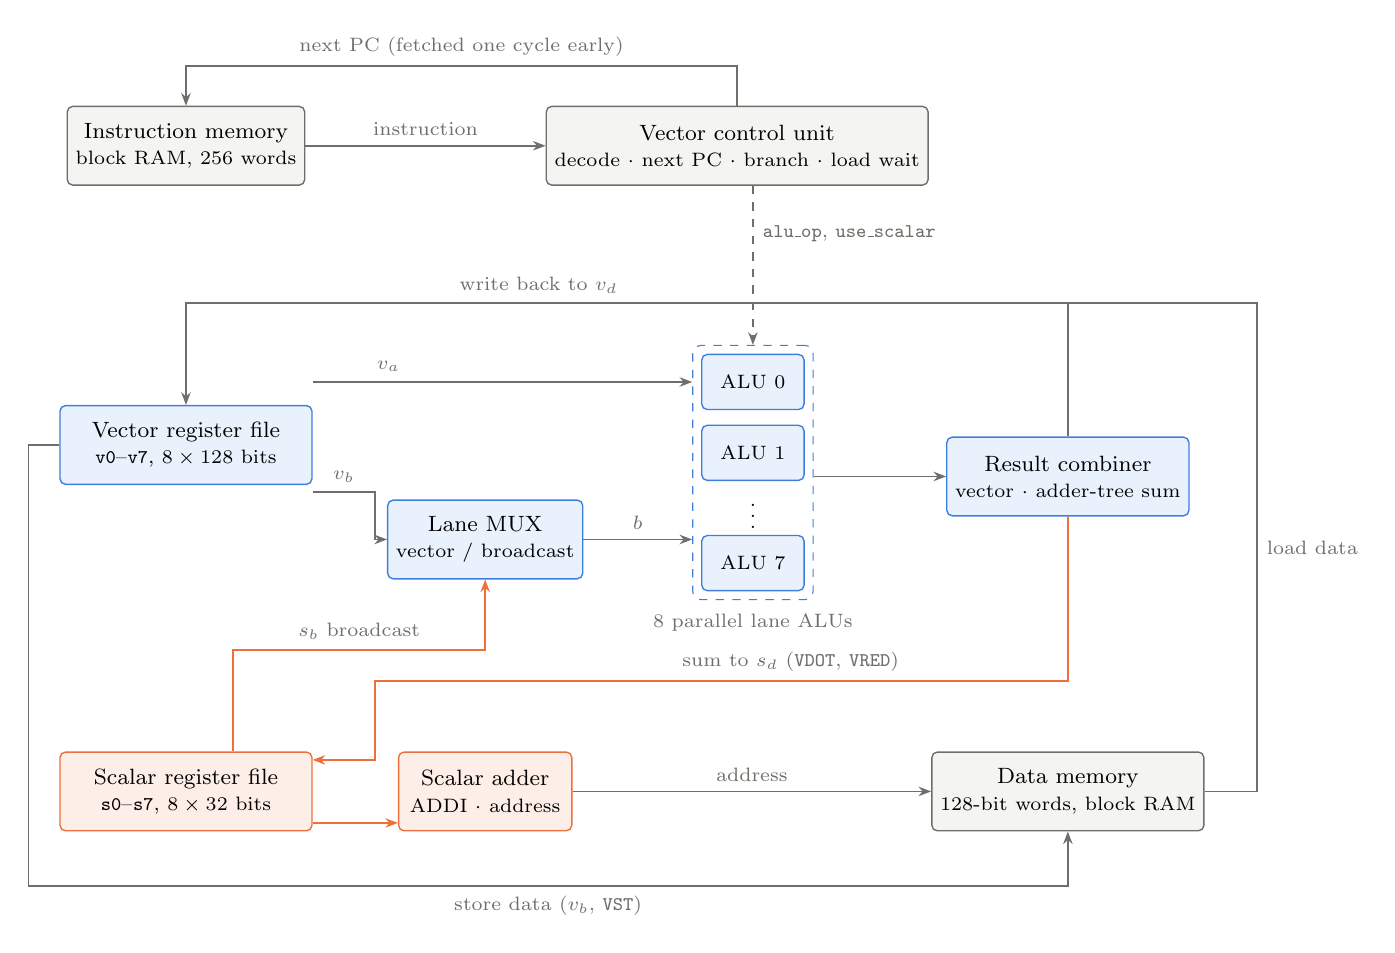
\begin{tikzpicture}[x=1mm, y=1mm, font=\footnotesize,
    blk/.style={box, minimum height=10mm, inner sep=3pt},
    vblk/.style={blk, fill=simdfill, draw=simd},
    sblk/.style={blk, fill=scalfill, draw=scal},
    gblk/.style={blk, fill=greyfill},
    lane/.style={box, fill=simdfill, draw=simd, minimum width=13mm, minimum height=7mm, font=\scriptsize},
    lbl/.style={note}]

% ---- Blocks ---------------------------------------------------------------------
\node[gblk, minimum width=30mm] (imem) at (0,8)     {Instruction memory\\\scriptsize block RAM, 256 words};
\node[gblk, minimum width=46mm] (ctrl) at (70,8)    {Vector control unit\\\scriptsize decode $\cdot$ next PC $\cdot$ branch $\cdot$ load wait};

\node[vblk, minimum width=32mm] (vrf)  at (0,-30)   {Vector register file\\\scriptsize \texttt{v0}--\texttt{v7}, $8 \times 128$ bits};
\node[vblk, minimum width=22mm] (mux)  at (38,-42)  {Lane MUX\\\scriptsize vector / broadcast};

\node[lane] (l0) at (72,-22) {ALU 0};
\node[lane] (l1) at (72,-31) {ALU 1};
\node[font=\scriptsize] at (72,-38) {$\vdots$};
\node[lane] (l7) at (72,-45) {ALU 7};
\begin{scope}[on background layer]
  \node[draw=simd, dashed, rounded corners=3pt, fit=(l0)(l7), inner sep=3pt] (lanes) {};
\end{scope}
\node[lbl, below=0.5mm] at (lanes.south) {8 parallel lane ALUs};

\node[vblk, minimum width=30mm] (comb) at (112,-34) {Result combiner\\\scriptsize vector $\cdot$ adder-tree sum};

\node[sblk, minimum width=32mm] (srf)  at (0,-74)   {Scalar register file\\\scriptsize \texttt{s0}--\texttt{s7}, $8 \times 32$ bits};
\node[sblk, minimum width=22mm] (sadd) at (38,-74)  {Scalar adder\\\scriptsize ADDI $\cdot$ address};
\node[gblk, minimum width=30mm] (dmem) at (112,-74) {Data memory\\\scriptsize 128-bit words, block RAM};

% ---- Fetch loop: the next address goes out one cycle early ----------------------
\draw[arr] (imem.east) -- node[above, lbl]{instruction} (ctrl.west);
\draw[arr] (ctrl.north) -- ++(0,5) -| node[pos=0.25, above, lbl]{next PC (fetched one cycle early)} (imem.north);

% ---- Control signals ---------------------------------------------------------------
\draw[arr, dashed] (ctrl.south -| lanes.north) -- node[right, lbl, pos=0.3]{\texttt{alu\_op}, \texttt{use\_scalar}} (lanes.north);

% ---- Vector datapath ------------------------------------------------------------------
\draw[arr] (vrf.east |- l0) -- node[above, lbl, pos=0.2]{$v_a$} (lanes.west |- l0);
\draw[arr] (vrf.east |- 0,-36) -- node[above, lbl]{$v_b$} (24,-36) |- (mux.west);
\draw[arr] (mux.east) -- node[above, lbl]{$b$} (lanes.west |- mux.east);
\draw[arr] (lanes.east |- comb.west) -- (comb.west);

% ---- Write-back: lane results or loaded data go into a vector register -----------
\draw[arr] (comb.north) -- (112,-12) -| node[pos=0.3, above, lbl]{write back to $v_d$} (vrf.north);
\draw[draw=edge, line width=0.6pt] (dmem.east) -- (136,-74) -- node[right, lbl, pos=0.5]{load data} (136,-12) -- (112,-12);

% ---- Scalar side -------------------------------------------------------------------------
\draw[arr, draw=scal] (srf.north -| 6,0) -- (6,-56) -- node[above, lbl, pos=0.5]{$s_b$ broadcast} (38,-56) -- (mux.south);
\draw[arr, draw=scal] (comb.south) -- (112,-60) -- node[above, lbl, pos=0.4]{sum to $s_d$ (\texttt{VDOT}, \texttt{VRED})} (24,-60) -- (24,-70) -- (srf.east |- 0,-70);
\draw[arr, draw=scal] (srf.east |- 0,-78) -- (sadd.west |- 0,-78);
\draw[arr] (sadd.east) -- node[above, lbl]{address} (dmem.west);
\draw[arr] (vrf.west) -- (-20,-30) -- (-20,-86) -- node[below, lbl, pos=0.5]{store data ($v_b$, \texttt{VST})} (112,-86) -- (dmem.south);
\end{tikzpicture}

\caption{Block diagram of the SIMD vector processing unit with eight lanes. Blue: vector
datapath; orange: scalar side; grey: control and memories; dashed: control signals. The
instruction and data memories are synchronous block RAM outside the core.}
\label{fig:block}
\end{figure*}

\textbf{Vector control unit.} Decodes each instruction into control signals and
computes the next program counter. Instruction memory is synchronous, so the unit sends
it the address of the \emph{next} instruction one cycle early, including the target of
a taken branch; branches therefore cost no extra cycle. A load takes two cycles: the
address goes out in the first while the program counter holds, and the returned data is
written in the second.

\textbf{Vector register file.} Eight $16L$-bit registers with two asynchronous read
ports and one synchronous write port.

\textbf{Scalar register file (scalar interface).} Eight 32-bit registers, with
\texttt{s0} hard-wired to zero. They hold addresses, loop counters, broadcast values and
reduction results. A third, debug read port exposes any register to the testbench, or to
the LEDs on the board.

\textbf{Lane multiplexers.} For each lane, operand B is either that lane's element of
$v_b$ or the low 16 bits of $s_b$ copied into every lane.

\textbf{Parallel ALUs.} $L$ copies of a combinational 14-operation lane ALU, created
with a \texttt{generate} loop and sharing one operation code. Lanes have no connection
to each other.

\textbf{Result combiner.} Passes the lane outputs on as one vector for write-back. For
reduce instructions it also sign-extends them to 32 bits and adds them in a
$\log_2 L$-level adder tree (Fig.~\ref{fig:combiner}), so the sum cannot overflow.

\textbf{FPGA top.} Adds block-RAM instruction and data memories loaded at power-up, a
power-on reset that holds the core for 15 clocks, a two-flip-flop synchroniser on the
reset button, three switches that select a scalar register and eight LEDs that show its
low byte.

\begin{figure}[t]
\centering
% Fig. 5 - the result combiner for 8 lanes. The lane results go straight on as
% one 128-bit vector; for reduce instructions they are also widened to 32 bits
% and added in pairs, log2(8) = 3 levels deep.
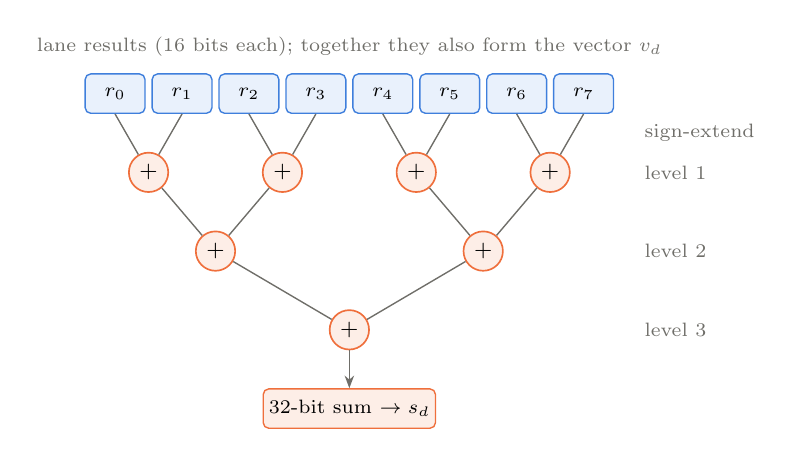
\begin{tikzpicture}[x=1mm, y=1mm, font=\scriptsize,
    res/.style={box, fill=simdfill, draw=simd, minimum width=7.6mm, minimum height=5mm, inner sep=0pt},
    add/.style={circle, draw=scal, fill=scalfill, line width=0.6pt, minimum size=5mm, inner sep=0pt, font=\footnotesize},
    wire/.style={draw=edge, line width=0.5pt}]

% Lane results r0..r7 (16 bits each).
\foreach \i in {0,...,7} \node[res] (r\i) at (\i*8.5, 30) {$r_{\i}$};
\node[note, anchor=south] at (29.75, 33.5) {lane results (16 bits each); together they also form the vector $v_d$};

% Level 1: four adders. Level 2: two. Level 3: one.
\foreach \j in {0,...,3} \node[add] (a\j) at (\j*17 + 4.25, 20) {$+$};
\foreach \j in {0,1}     \node[add] (b\j) at (\j*34 + 12.75, 10) {$+$};
\node[add] (c0) at (29.75, 0) {$+$};

\foreach \j [evaluate=\j as \p using int(2*\j), evaluate=\j as \q using int(2*\j+1)] in {0,...,3} {
  \draw[wire] (r\p.south) -- (a\j); \draw[wire] (r\q.south) -- (a\j);
}
\draw[wire] (a0) -- (b0); \draw[wire] (a1) -- (b0);
\draw[wire] (a2) -- (b1); \draw[wire] (a3) -- (b1);
\draw[wire] (b0) -- (c0); \draw[wire] (b1) -- (c0);

\node[box, fill=scalfill, draw=scal, minimum height=5mm] (sum) at (29.75, -10) {32-bit sum $\rightarrow s_d$};
\draw[arr] (c0) -- (sum);

% Level labels on the right.
\foreach \y/\t in {25/sign-extend, 20/level 1, 10/level 2, 0/level 3}
  \node[note, anchor=west] at (66, \y) {\t};

\end{tikzpicture}

\caption{Result combiner for eight lanes. Reduce instructions widen each lane result to
32 bits and sum them in $\log_2 8 = 3$ levels of adders; vector instructions use the
lane results directly as the destination vector.}
\label{fig:combiner}
\end{figure}

\subsection{Timing Model}
Every instruction except \texttt{VLD} completes in one cycle (Fig.~\ref{fig:timing}),
so the run time of a program is
\begin{equation}
  \text{cycles} = \text{instructions} + \text{loads}.
  \label{eq:cycles}
\end{equation}
For a kernel with $k$ set-up instructions, a loop body of $b$ instructions containing
$\ell$ loads, and $N$ elements on $L$ lanes,
\begin{equation}
  C(L) = k + \frac{N}{L}\,(b + \ell) + 1, \qquad
  S(L) = \frac{C(1)}{C(L)} < L,
  \label{eq:model}
\end{equation}
where the final 1 is \texttt{HALT}. The speed-up $S$ approaches $L$ as $N$ grows; the
$k + 1$ serial instructions are the Amdahl term.

\begin{figure}[t]
\centering
% Fig. 6 - one pass of the vadd loop, cycle by cycle (from vec_control_unit.v).
% Each VLD takes two cycles; the taken BNE costs nothing because the control
% unit already sends the branch target (2) to instruction memory in cycle 7.
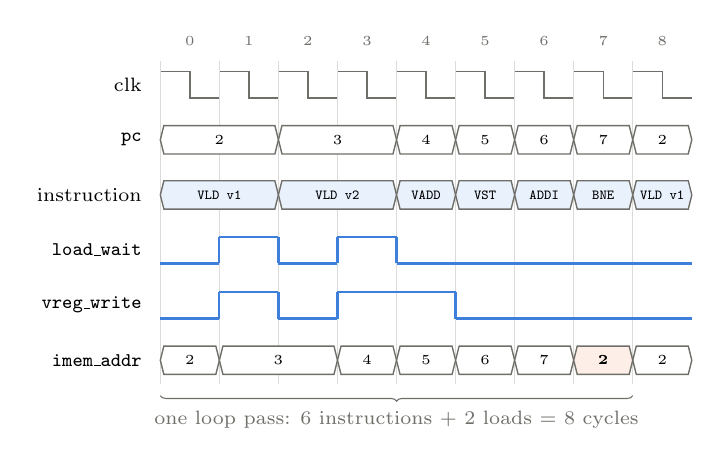
\begin{tikzpicture}[x=7.5mm, y=1mm, font=\tiny,
    sig/.style={draw=edge, line width=0.5pt},
    hi/.style={draw=simd, line width=0.8pt}]

% sigbus <first cycle> <last cycle + 1> <row y> <text> <fill colour>
\newcommand{\sigbus}[5]{%
  \filldraw[sig, fill=#5] ({#1+0.06},{#3+1.8}) -- ({#2-0.06},{#3+1.8}) -- ({#2},{#3}) --
      ({#2-0.06},{#3-1.8}) -- ({#1+0.06},{#3-1.8}) -- ({#1},{#3}) -- cycle;
  \node at ({(#1+#2)/2},{#3}) {#4};}
% sigbit <row y> <list of 0/1 values, one per cycle>
\newcommand{\sigbit}[2]{%
  \foreach \v [count=\c from 0] in {#2} {
    \pgfmathsetmacro{\h}{#1+\v*3.4-1.7}
    \draw[hi] (\c,\h) -- (\c+1,\h);
  }}

% Signal names.
\foreach \y/\t in {30/clk, 23/\texttt{pc}, 16/instruction, 9/\texttt{load\_wait}, 2/\texttt{vreg\_write}, -5/\texttt{imem\_addr}}
  \node[anchor=east, font=\scriptsize] at (-0.15,\y) {\t};

% Cycle numbers and the clock.
\foreach \c in {0,...,8} {
  \node[text=edge] at (\c+0.5, 35.5) {\c};
  \draw[sig] (\c,28.3) -- (\c,31.7) -- (\c+0.5,31.7) -- (\c+0.5,28.3) -- (\c+1,28.3);
  \draw[edge!25, line width=0.3pt] (\c,-8) -- (\c,33);
}

% Program counter, instruction and next-address buses.
\foreach \a/\b/\t in {0/2/2, 2/4/3, 4/5/4, 5/6/5, 6/7/6, 7/8/7, 8/9/2} {\sigbus{\a}{\b}{23}{\t}{white}}
\foreach \a/\b/\t in {0/2/{VLD v1}, 2/4/{VLD v2}, 4/5/VADD, 5/6/VST, 6/7/ADDI, 7/8/BNE, 8/9/{VLD v1}}
  {\sigbus{\a}{\b}{16}{\texttt{\t}}{simdfill}}
\foreach \a/\b/\t in {0/1/2, 1/3/3, 3/4/4, 4/5/5, 5/6/6, 6/7/7, 8/9/2} {\sigbus{\a}{\b}{-5}{\t}{white}}
\sigbus{7}{8}{-5}{\textbf{2}}{scalfill}

% One-bit signals.
\sigbit{9}{0,1,0,1,0,0,0,0,0}
\sigbit{2}{0,1,0,1,1,0,0,0,0}
\foreach \c in {1,2,3,4} \draw[hi] (\c,7.3) -- (\c,10.7);   % load_wait edges
\foreach \c in {1,2,3,5} \draw[hi] (\c,0.3) -- (\c,3.7);    % vreg_write edges

% What one pass costs.
\draw[decorate, decoration={brace, amplitude=2pt, mirror}, edge] (0,-9.5) -- node[below=2pt, font=\scriptsize, text=edge]
  {one loop pass: 6 instructions + 2 loads = 8 cycles} (8,-9.5);
\end{tikzpicture}

\caption{One pass of the vector-add loop at the cycle level. Each \texttt{VLD} holds the
program counter for one cycle and writes its register in the second. In cycle 7 the
taken \texttt{BNE} already sends the loop start (address 2, orange) to instruction
memory, so the branch costs nothing.}
\label{fig:timing}
\end{figure}

\subsection{Software Tool Flow}\label{sec:tools}
\textbf{Assembler.} A two-pass assembler (\texttt{vasm.py}) resolves labels in the
first pass and encodes in the second. It accepts named constants such as \texttt{ITER},
chooses the vector--vector or vector--scalar form from the third operand, and reports
errors with their line numbers.

\textbf{Golden model.} An instruction-level simulator (\texttt{golden.py}) executes the
assembled words with the same wrap-around rules as the hardware and predicts the final
data memory, the scalar registers, the instruction count and the cycle count
from~\eqref{eq:cycles}. It shares no code with the RTL.

\textbf{Workload runner.} For each program and lane count, \texttt{run\_workloads.py}
generates input data with a fixed seed, assembles the program with
$\mathit{ITER} = N/L$, runs the golden model and the RTL simulation, compares them and
writes the cycle counts to a CSV file.

\subsection{Verification Methodology}\label{sec:verif}
Verification works in layers (Table~\ref{tab:verif}). Unit testbenches drive each block
with corner cases and seeded random stimulus and compare it against reference models
written independently of the RTL (for example, shifts as multiplication or division by
$2^n$); the ALU test also counts the true and false outcomes of each compare and fails
on any coverage hole. The system testbench loads a program and its data, runs the core
to \texttt{HALT}, keeps the clock running for 50 more cycles (no memory write is
allowed) and then compares every data-memory word, every scalar register (through the
debug port), every vector register and both counters with the golden model. The golden-model result is
itself checked against plain arithmetic, such as $C_i = A_i + B_i$, which catches
errors in the programs. Directed programs exercise what the benchmarks never do:
writes to \texttt{s0}, address and program-counter wrap-around, back-to-back loads, a
branch into a load, a 32-bit scalar broadcast, every unused opcode, branches on numbers
that differ only in bit 16 or bit 31, unused instruction fields filled in, and
instructions after \texttt{HALT} that must never run. Random programs go further: a
fuzzer generates programs with every opcode, random register fields, branches,
addresses and memory contents, and each must match the golden model. The board check
simulates the FPGA top exactly as built, started only by its power-on reset, and
compares its registers and all of its data memory. Finally, mutation tests inject bugs
and require the tests to fail. A sixth program,
\texttt{isa\_test}, runs all 42 vector-ALU and reduce forms on random data, so every
instruction is exercised on the complete core. Continuous integration repeats the lint
and the tests on every change to the repository.

\begin{table}[t]
\centering
\caption{Verification Plan}
\label{tab:verif}
\footnotesize
\setlength{\tabcolsep}{4pt}
\renewcommand{\arraystretch}{1.12}
\begin{tabular}{lL{0.45\columnwidth}r}
\toprule
Testbench & What it checks & Checks \\
\midrule
\texttt{tb\_vec\_alu}       & 14 jobs, 8 lanes: corner-value pairs, every shift, no carry between lanes, 2,000 random vectors per job & 225,496 \\
\texttt{tb\_regfiles}       & all registers and ports, write enable, read during write, \texttt{s0} = 0 & 10,044 \\
\texttt{tb\_lane\_combiner} & broadcast and vector modes; sums at extreme values; $L = 1, 2, 4, 8$ & $4 \times 11{,}008$ \\
\texttt{tb\_simd\_core}     & 6 programs: memory, all registers, cycles; no write after \texttt{HALT} & 24 runs \\
directed tests              & corner-case programs, same testbench & 12 runs \\
random programs             & every opcode; random fields, branches, data & 4,000 \\
\texttt{tb\_fpga\_top}      & board version, \texttt{isa\_test}, from power-on: registers, memory & 4 builds \\
software tests              & encodings, branches, errors, model corners & 11 \\
\bottomrule
\end{tabular}
\end{table}

\subsection{Workloads and Experimental Setup}
Five kernels (Table~\ref{tab:kernels}) run on $N = 256$ random 16-bit integers over the
full range, drawn with a fixed seed. The plain-arithmetic checks wrap each result to 16
bits as the hardware does (for \texttt{VDOT}, each product keeps its low 16 bits). The
cycle counts do not depend on the data, because no kernel branches on it. Threshold is a branch-free conditional: a compare builds a mask, an
\texttt{XOR} with all ones inverts it and an \texttt{AND} applies it. Simulation uses
Icarus Verilog~13 (12 in continuous integration), lint uses Verilator~5 with all
warnings enabled, and synthesis uses
Yosys~0.70 for a Lattice ECP5 LFE5U-25F (speed grade 6) with place-and-route in
nextpnr-ecp5~0.11. The FPGA builds are loaded with \texttt{isa\_test}, which uses every instruction: a
program that left an instruction class unused would let synthesis remove its logic and
make the design look smaller and faster. Each ECP5 build is placed with three seeds,
and the median of the maximum frequency $F_{\max}$ estimated by nextpnr's static
timing analysis is given. A Yosys estimate for the Xilinx Artix-7 xc7a35t of the
Basys-3 board, flattened like the ECP5 build, is also reported.

\begin{table}[t]
\centering
\caption{Benchmark Kernels: Set-up Instructions $k$, Loop Body $b$ and Loads $\ell$}
\label{tab:kernels}
\footnotesize
\begin{tabular}{llrrr}
\toprule
Kernel & Operation & $k$ & $b$ & $\ell$ \\
\midrule
vadd      & $C_i = A_i + B_i$                      & 2 & 6 & 2 \\
saxpy     & $Y_i = a X_i + Y_i$                    & 3 & 7 & 2 \\
relu      & $Y_i = \max(X_i, 0)$                   & 2 & 5 & 1 \\
threshold & $Y_i = X_i$ if $X_i \ge T$, else 0     & 4 & 7 & 1 \\
dot       & $s = \sum_i A_i B_i$                   & 3 & 6 & 2 \\
\bottomrule
\end{tabular}
\end{table}

% =============================================================================
\section{Prototype Results}\label{sec:results}

\subsection{Verification}
All unit tests pass. All 24 system runs (six programs at four lane counts), all 12
directed runs and 4,000 random programs (1,000 per lane count) match the golden model
exactly in memory contents, scalar and vector registers, instruction count and cycle
count, and the board version matches it in its registers and all 1,024 memory words at
every lane count. Verilator lint with all warnings enabled reports nothing for any
module; the only two waivers mark bits that are unused on purpose. Every injected
mutation was detected (Table~\ref{tab:mutation}).

\begin{table}[t]
\centering
\caption{Mutation Tests: Injected Bugs and the Test That Caught Each}
\label{tab:mutation}
\footnotesize
\setlength{\tabcolsep}{3pt}
\begin{tabular}{L{0.42\columnwidth}ll}
\toprule
Injected bug & Caught by & Result \\
\midrule
\texttt{SRA} made a logical shift & \texttt{tb\_vec\_alu} & negative inputs \\
adder tree pairs the wrong lanes & \texttt{tb\_lane\_combiner} & 5,002 errors \\
no wait for load data & \texttt{tb\_simd\_core} & every result \\
zero- not sign-extension ($L = 1$) & \texttt{tb\_lane\_combiner} & 2,507 errors \\
code after \texttt{HALT} keeps running & directed & memory, regs \\
\texttt{BNE} ignores bits 16--31 & directed & memory \\
\texttt{VST}/\texttt{BNE}/\texttt{HALT} write a reg. & \texttt{tb\_simd\_core} & vector regs \\
FPGA stores to a wrong address & \texttt{tb\_fpga\_top} & stored words \\
\bottomrule
\end{tabular}
\end{table}

\subsection{Scalar Versus SIMD}
Table~\ref{tab:perf} gives the cycle counts. Every one of the 20 kernel counts equals
the prediction of~\eqref{eq:model} exactly. At eight lanes the speed-up is
$7.87$--$7.92\x$, 1.0--1.7\% below the ideal $8\x$ (mean $7.89\x$), and halving the
lane count halves the gain (Fig.~\ref{fig:perf}, left and centre). The shortfall is the
two to four set-up instructions and \texttt{HALT}, which run once whatever the lane
count, so it grows with the ratio of serial instructions to loop work: threshold, with
four set-up instructions, loses most (1.7\%), and vadd, with two set-up instructions
and eight cycles per pass, loses least (1.0\%).

\begin{table}[t]
\centering
\caption{Clock Cycles for $N = 256$ Elements}
\label{tab:perf}
\footnotesize
\begin{tabular}{lrrrrr}
\toprule
Kernel & $L{=}1$ & $L{=}2$ & $L{=}4$ & $L{=}8$ & Speed-up \\
\midrule
vadd      & 2051 & 1027 & 515 & 259 & $7.92\x$ \\
saxpy     & 2308 & 1156 & 580 & 292 & $7.90\x$ \\
relu      & 1539 &  771 & 387 & 195 & $7.89\x$ \\
threshold & 2053 & 1029 & 517 & 261 & $7.87\x$ \\
dot       & 2052 & 1028 & 516 & 260 & $7.89\x$ \\
\bottomrule
\end{tabular}
\end{table}

\begin{figure*}[t]
\centering
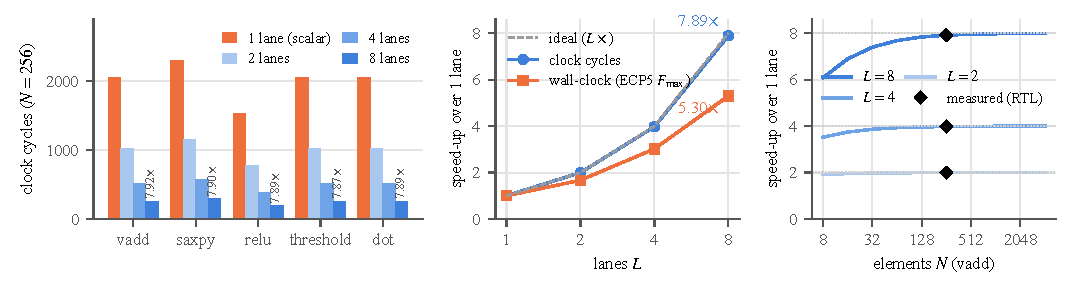
\includegraphics[width=\textwidth]{figures/perf.pdf}
\caption{Scalar versus SIMD. Left: clock cycles per kernel at 1, 2, 4 and 8 lanes, with
the eight-lane speed-up. Centre: mean speed-up over the five kernels in cycles and in
wall-clock time (with each build's ECP5 $F_{\max}$); dashed: ideal. Right: vadd speed-up
against $N$ from~\eqref{eq:model}; diamonds: RTL measurements at $N = 256$.}
\label{fig:perf}
\end{figure*}

Because~\eqref{eq:model} matches every run, it predicts the speed-up at other array
sizes (Fig.~\ref{fig:perf}, right). For vadd at eight lanes it is $6.1\x$ at $N = 8$,
$7.9\x$ at $N = 256$ and $7.99\x$ at $N = 4096$ (sizes above 341 elements do not fit
the scalar build's memory, so they are predicted, not run): the serial part is fixed, so longer
arrays hide it, as Gustafson~\cite{gustafson} observed for scaled problems. At
$N = 256$ eight lanes complete 0.88 (saxpy) to 1.31 (relu) elements per clock cycle,
against 0.11 to 0.17 for one lane.

\subsection{FPGA Resources and Clock Frequency}
Table~\ref{tab:fpga} and Fig.~\ref{fig:fpga} give the synthesis results. Each lane adds one hardware multiplier and its own ALU, about 550
logic cells per added lane on average from one to eight lanes. Shared logic (control,
scalar registers, memories) is paid once, so eight lanes need $3.5\x$ the logic of one,
not $8\x$. Yosys maps both register files to distributed LUT RAM, so the ECP5 build
uses only 16 flip-flops at every lane count (the program counter, the load and halt
flags and the reset logic); block RAM grows from two to nine blocks because the data
words widen with $L$. On the Artix-7, Yosys estimates 2,731 LUTs (13\%) and eight DSP
slices, one per lane, for eight lanes. 

\begin{table}[t]
\centering
\caption{FPGA Results. ECP5-25F After Place-and-Route ($F_{\max}$: Median and Range of
Three Seeds); Artix-7 xc7a35t Yosys Estimate}
\label{tab:fpga}
\footnotesize
\setlength{\tabcolsep}{3pt}
\begin{tabular}{rrrrrrrr}
\toprule
 & \multicolumn{5}{c}{ECP5-25F} & \multicolumn{2}{c}{Artix-7} \\
\cmidrule(lr){2-6}\cmidrule(lr){7-8}
$L$ & Cells & FF & Mult. & BRAM & $F_{\max}$ (MHz) & LUTs & DSP \\
\midrule
1 & 1,555 (6.4\%)  & 16 & 1 & 2 & 43.3 (42.0--44.3) &   548 & 1 \\
2 & 1,943 (8.0\%)  & 16 & 2 & 3 & 36.2 (36.1--37.2) &   864 & 2 \\
4 & 3,720 (15.3\%) & 16 & 4 & 5 & 32.9 (32.7--33.7) & 1,483 & 4 \\
8 & 5,396 (22.2\%) & 16 & 8 & 9 & 29.1 (28.9--29.8) & 2,731 & 8 \\
\bottomrule
\end{tabular}
\end{table}

\begin{figure*}[t]
\centering
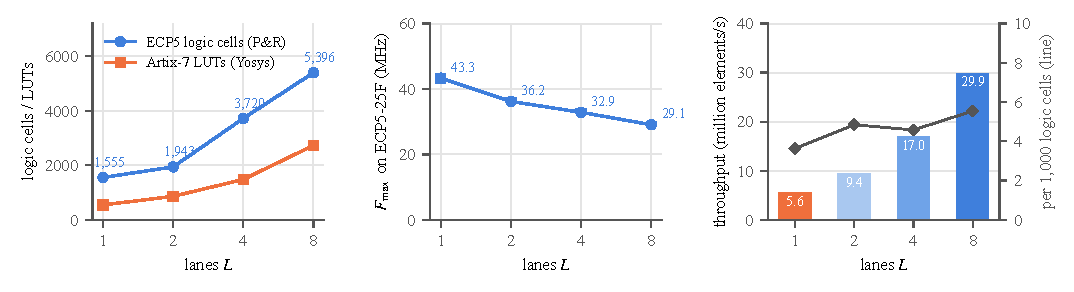
\includegraphics[width=\textwidth]{figures/fpga.pdf}
\caption{FPGA scaling with every instruction in use. Left: logic on the ECP5-25F after
place-and-route and on the Artix-7 (Yosys estimate). Centre: ECP5 $F_{\max}$, median of
three seeds (bars: range). Right: throughput, mean elements per cycle times $F_{\max}$
(bars), and the same per 1,000 logic cells (line).}
\label{fig:fpga}
\end{figure*}

The estimated maximum frequency falls from 43.3~MHz at one lane to 29.1~MHz at eight,
33\% lower; the spread between placement seeds is at most 2.3~MHz. Because the core
executes each instruction in a single cycle, its critical path crosses the whole
datapath. At eight lanes nextpnr reports it from the instruction block RAM through the
scalar and vector register reads, a lane ALU (the multiplier in two of the three
placements), the result selection and the adder tree to the scalar register write.
Wider designs also spread over more of the device, which lengthens the routing.

\subsection{Throughput and Area Efficiency}
Combining cycles and clock, the eight-lane unit finishes a kernel $7.89 \times
29.1/43.3 = 5.3\x$ sooner than the scalar build, against $1.7\x$ for two lanes and
$3.0\x$ for four (Fig.~\ref{fig:perf}, centre). Throughput rises from 5.6 to 9.4, 17.0
and 29.9 million elements per second (Fig.~\ref{fig:fpga}, right). Per 1,000 logic cells it grows from 3.6 million elements per second at one lane to
5.5 at eight: eight lanes do 1.5 times
as much work per cell as one, because the shared logic is spread over more lanes.

% =============================================================================
\section{Discussion and Limitations}\label{sec:discussion}

\textbf{Near-ideal scaling in cycles.} The lanes never interact, the core has no
hazards, and every kernel's serial part is three to five instructions, so the cycle
speed-up is within 1.7\% of ideal and is predicted exactly by~\eqref{eq:model}. The
unit therefore demonstrates the main promise of SIMD: the work done per instruction
grows with the number of lanes while the control cost does not.

\textbf{The clock pays for the width.} Single-cycle execution makes the design simple
to verify and its timing exact, but puts the multiplier and the adder tree on the same
path as the instruction fetch and the register write. A third of the clock is lost
between one and eight lanes, so a wider single-cycle datapath delivers less than its
cycle count suggests; pipelining is needed to keep the clock rate.

\textbf{The loop, not the ALU, sets the pace.} In one pass of vadd at eight lanes only
one of the eight cycles does arithmetic; two loads take four cycles, and the store and
the loop control take three (Fig.~\ref{fig:timing}). The ALUs are idle most of the time. Memory bandwidth is not the limit, since
the block RAM could deliver a 128-bit word every cycle; the limit is issue: one
instruction per cycle, loads that take two cycles and are not overlapped, and the loop
control. Loop unrolling, auto-incrementing addresses or pipelined loads would raise
throughput without adding lanes.

\textbf{Limitations and threats to validity.}
\begin{itemize}
\item The design is not pipelined, so the clock frequencies are those of a single-cycle
      datapath and understate what the lane array could reach.
\item Elements are 16-bit integers only, with wrap-around and no saturation, and there
      is no masked (predicated) execution; conditionals use \texttt{AND} masks.
\item \texttt{VDOT} keeps only the low 16 bits of each product, so its inputs must be
      small enough for the products to fit, as in the dot-product test; a widening
      multiply would remove this limit.
\item A program must be reassembled for each lane count, because the loop count
      $N/L$ is a constant; there is no \texttt{vsetvli}-style instruction.
\item The FPGA results are for one device and speed grade, and $F_{\max}$ is nextpnr's
      static-timing estimate without pin constraints. Artix-7 figures are Yosys
      estimates without timing, and the Vivado flow for the Basys-3 board is written but
      not yet run. The board check simulates the FPGA top; the design has not yet run on
      a physical board.
\item The kernels are short and regular. No power or energy was measured.
\end{itemize}

% =============================================================================
\section{Conclusion and Phase II Plan}\label{sec:conclusion}
The Phase~I prototype is complete and verified. An eight-lane, 128-bit SIMD unit
executes a 48-instruction ISA, matches its golden model cycle for cycle at every lane
count, and reaches a $7.9\x$ cycle speed-up and a $5.3\x$ wall-clock speed-up over its
own scalar configuration on a mid-range FPGA, at 22\% of the logic. The results show
where the remaining performance lies: in the clock, which a pipeline would recover, and
in the loop overhead around the arithmetic. Phase~II will therefore
(i)~pipeline the core to raise $F_{\max}$ and recover wall-clock speed-up;
(ii)~measure exact Artix-7 resources and timing in Vivado and run the design on a
Basys-3 board;
(iii)~add predicated (masked) execution and saturating arithmetic;
(iv)~reduce loop overhead with unrolling and auto-incrementing addresses, and measure
speed-up against problem size on the hardware; and
(v)~compare estimated power per operation for the scalar and SIMD builds.

% =============================================================================
\section*{Code and Data Availability}
All RTL, testbenches, programs, scripts, results and figures are in the repository
named on the first page. One command,
\texttt{make test}, runs the lint, the unit testbenches, the software tests, the system
and directed runs, 100 random programs and the board check; \texttt{make fuzz} runs
4,000 random programs; \texttt{make perf} and \texttt{make syn} regenerate the cycle
counts and the FPGA results, and \texttt{make report} rebuilds the figures and this
paper from them. 

\section*{Individual Contributions}
\textbf{Mahir Abdullah} (lead): the architecture, instruction format and block interfaces
that the team built against; the vector control unit with early instruction fetch and
two-cycle load; core integration with performance counters; the instruction-level golden
model, the workload runner, the directed tests and the random-program fuzzer; the
system testbench; the repository,
continuous integration and documentation; and this report.

\textbf{Krishiv Gupta}: the 14-operation lane ALU and its \texttt{generate}-based array,
including signed and unsigned compares and arithmetic shifts, with its 225,496-check testbench, which also confirms that no carry crosses a lane; the FPGA top with
block-RAM memories and power-on reset; the board check; the ECP5 and Artix-7 synthesis
sweep, the Vivado script and Basys-3 constraints; and the resource and $F_{\max}$
analysis.

\textbf{Abhiman Singh}: the vector and scalar register files, with two read ports and
one write port each, a hard-wired zero register and the debug port that forms the scalar
interface; and their testbench, which covers read-during-write behaviour and random
cycles against a shadow model.

\textbf{Gogulamudi Jayadeep}: the lane multiplexers and the result combiner with its $\log_2 L$
adder tree, verified for every lane count; and the scalar-versus-SIMD analysis: cycle
counts for 1, 2, 4 and 8 lanes, speed-up, elements per cycle and the figures.

\textbf{Ashish Kushwaha}: the two-pass assembler with labels, constants and
line-numbered error messages, and its tests; and the six workload programs, including
the branch-free threshold kernel and the instruction-coverage program.

\section*{Acknowledgment}
The authors thank the developers of Icarus Verilog, Verilator, Yosys and nextpnr, whose
open tools make every result in this report reproducible.

% =============================================================================
% References are numbered in the order they are first cited.
\begin{thebibliography}{99}

\bibitem{cray1} R.~M. Russell, ``The CRAY-1 computer system,''
\emph{Commun. ACM}, vol.~21, no.~1, pp.~63--72, Jan. 1978.

\bibitem{mmx} A.~Peleg and U.~Weiser, ``MMX technology extension to the Intel
architecture,'' \emph{IEEE Micro}, vol.~16, no.~4, pp.~42--50, Aug. 1996,
doi: 10.1109/40.526924.

\bibitem{hp6} J.~L. Hennessy and D.~A. Patterson, \emph{Computer Architecture: A
Quantitative Approach}, 6th~ed. Cambridge, MA, USA: Morgan Kaufmann, 2017, ch.~4.

\bibitem{flynn72} M.~J. Flynn, ``Some computer organizations and their effectiveness,''
\emph{IEEE Trans. Comput.}, vol.~C-21, no.~9, pp.~948--960, Sep. 1972.

\bibitem{espasa98} R.~Espasa, M.~Valero, and J.~E. Smith, ``Vector architectures:
Past, present and future,'' in \emph{Proc. 12th Int. Conf. Supercomputing (ICS)},
1998, pp.~425--432.

\bibitem{sse} S.~K. Raman, V.~Pentkovski, and J.~Keshava, ``Implementing streaming
SIMD extensions on the Pentium III processor,'' \emph{IEEE Micro}, vol.~20, no.~4,
pp.~47--57, Jul. 2000, doi: 10.1109/40.865866.

\bibitem{viram} C.~E. Kozyrakis and D.~A. Patterson, ``Scalable vector processors
for embedded systems,'' \emph{IEEE Micro}, vol.~23, no.~6, pp.~36--45, Nov. 2003,
doi: 10.1109/MM.2003.1261385.

\bibitem{asanovic98} K.~Asanovi\'c, ``Vector microprocessors,'' Ph.D. dissertation,
Univ. California, Berkeley, CA, USA, 1998.

\bibitem{maven} Y.~Lee, R.~Avizienis, A.~Bishara, R.~Xia, D.~Lockhart, C.~Batten,
and K.~Asanovi\'c, ``Exploring the tradeoffs between programmability and efficiency
in data-parallel accelerators,'' in \emph{Proc. 38th Int. Symp. Comput. Archit.
(ISCA)}, 2011, pp.~129--140.

\bibitem{rvv} RISC-V International, ``The RISC-V `V' vector extension,''
version~1.0, 2021. [Online]. Available: \url{https://github.com/riscv/riscv-v-spec}

\bibitem{sve} N.~Stephens \emph{et al.}, ``The ARM scalable vector extension,''
\emph{IEEE Micro}, vol.~37, no.~2, pp.~26--39, Mar. 2017, doi: 10.1109/MM.2017.35.

\bibitem{ara} M.~Cavalcante, F.~Schuiki, F.~Zaruba, M.~Schaffner, and L.~Benini,
``Ara: A 1-GHz+ scalable and energy-efficient RISC-V vector processor with
multiprecision floating-point support in 22-nm FD-SOI,'' \emph{IEEE Trans. Very
Large Scale Integr. (VLSI) Syst.}, vol.~28, no.~2, pp.~530--543, Feb. 2020.

\bibitem{intelsdm} Intel Corp., \emph{Intel 64 and IA-32 Architectures Software
Developer's Manual}, vol.~2. [Online]. Available: \url{https://www.intel.com/sdm}.
Accessed: Nov. 6, 2026.

\bibitem{armarm} Arm Ltd., \emph{Arm Architecture Reference Manual for A-profile
Architecture}. [Online]. Available:
\url{https://developer.arm.com/documentation/ddi0487/latest}. Accessed: Nov. 6, 2026.

\bibitem{msa} MIPS Technologies, ``MIPS SIMD Architecture,'' white paper, rev.~1.00, 2012.

\bibitem{vespa} P.~Yiannacouras, J.~G. Steffan, and J.~Rose, ``VESPA: Portable,
scalable, and flexible FPGA-based vector processors,'' in \emph{Proc. Int. Conf.
Compilers, Archit. Synth. Embedded Syst. (CASES)}, 2008, pp.~61--70.

\bibitem{vipers} J.~Yu, C.~Eagleston, C.~H.-Y. Chou, M.~Perreault, and G.~Lemieux,
``Vector processing as a soft processor accelerator,'' \emph{ACM Trans.
Reconfigurable Technol. Syst.}, vol.~2, no.~2, pp.~12:1--12:34, 2009,
doi: 10.1145/1534916.1534922.

\bibitem{vegas} C.~H. Chou, A.~Severance, A.~D. Brant, Z.~Liu, S.~Sant, and
G.~G.~F. Lemieux, ``VEGAS: Soft vector processor with scratchpad memory,'' in
\emph{Proc. ACM/SIGDA Int. Symp. Field Program. Gate Arrays (FPGA)}, 2011,
pp.~15--24.

\bibitem{mxp} A.~Severance and G.~G.~F. Lemieux, ``Embedded supercomputing in
FPGAs with the VectorBlox MXP matrix processor,'' in \emph{Proc. Int. Conf.
Hardware/Software Codesign Syst. Synth. (CODES+ISSS)}, 2013, pp.~1--10,
doi: 10.1109/CODES-ISSS.2013.6658993.

\bibitem{vicuna} M.~Platzer and P.~Puschner, ``Vicuna: A timing-predictable RISC-V
vector coprocessor for scalable parallel computation,'' in \emph{Proc. 33rd Euromicro
Conf. Real-Time Syst. (ECRTS)}, ser. LIPIcs, vol.~196, 2021, pp.~1:1--1:18,
doi: 10.4230/LIPIcs.ECRTS.2021.1.

\bibitem{amdahl} G.~M. Amdahl, ``Validity of the single processor approach to
achieving large scale computing capabilities,'' in \emph{Proc. AFIPS Spring Joint
Comput. Conf.}, 1967, pp.~483--485.

\bibitem{gustafson} J.~L. Gustafson, ``Reevaluating Amdahl's law,'' \emph{Commun.
ACM}, vol.~31, no.~5, pp.~532--533, May 1988.

\bibitem{demillo} R.~A. DeMillo, R.~J. Lipton, and F.~G. Sayward, ``Hints on test data
selection: Help for the practicing programmer,'' \emph{Computer}, vol.~11, no.~4,
pp.~34--41, Apr. 1978.

\bibitem{icarus} S.~Williams, ``Icarus Verilog,'' 2026. [Online]. Available:
\url{https://steveicarus.github.io/iverilog/}

\bibitem{verilator} W.~Snyder, ``Verilator,'' 2026. [Online]. Available:
\url{https://www.veripool.org/verilator/}

\bibitem{yosys} C.~Wolf, ``Yosys Open SYnthesis Suite.'' [Online]. Available:
\url{https://yosyshq.net/yosys/}

\bibitem{nextpnr} D.~Shah, E.~Hung, C.~Wolf, S.~Bazanski, D.~Gisselquist, and
M.~Milanovi\'c, ``Yosys+nextpnr: An open source framework from Verilog to bitstream
for commercial FPGAs,'' in \emph{Proc. IEEE 27th Annu. Int. Symp.
Field-Program. Custom Comput. Mach. (FCCM)}, 2019, arXiv:1903.10407.

\bibitem{ieee1364} \emph{IEEE Standard for Verilog Hardware Description Language},
IEEE Std 1364-2005, 2006.

\end{thebibliography}

\end{document}
